The simulation is broken up into five modules: geometry, hydrodynamics, dynamics and control, structures, and economics.
The geometry module uses both bulk dimensions and structural thicknesses to calculate relevant areas, volumes, masses, measures of center, hydrostatics, and stability margins.
Hydrodynamics uses the bulk dimensions to calculate hydrodynamic coefficients using a semi-analytical method.
The dynamics and control module uses the mass, hydrodynamic coefficients, and generator ratings to determine the loads, response amplitude, and power production using a linear frequency domain model adapted to handle specific nonlinearities including drag and powertrain saturation behavior.
It considers both operational and storm design load cases.
The structures module takes in these loads along with bulk dimensions and structural thicknesses to calculate the stress and factor of safety to various failure criterion.
Finally, the economics module calculates the PTO and structural capital costs from generator ratings and material usage respectively, and combines it with the power matrix to estimate the levelized cost of energy.

The extended design structure matrix (XDSM) diagram in Figure \ref{fig:n2} illustrates the functional interfaces between modules.
XDSM diagrams are standard in MDO, with more details available in \cite{lambe_extensions_2012}.
Variables above and below each module are inputs, and variables to the left and right are outputs.
Design variables are shown in the first row.
The optimizer uses the objective $J$ and constraint $g$ outputs from a simulation run to inform the next iteration of design variables $x$, iterating until ultimately converging to a set of optimal values $x^*$, $J^*$, and $g^*$.

\paragraph{Absence of Feedback Coupling}
The lack of variables in the lower left portion of the diagram indicates that there is no feedback coupling between modules, so an external solver to enforce consistency is not necessary.
This helps decrease the simulation computation time.
\paragraph{Presence of Feed-Forward Coupling}
The presence of variables in the upper right of the diagram indicates feed-forward coupling in which the output of one module directly affects subsequent modules.
\begin{figure}
\centering
\includegraphics[width=\linewidth]{\matlabFilepath{3}}
\caption{Simplified $N^2$/XDSM diagram}\label{fig:n2}
\end{figure}
When coupling is \textit{non-monotonic}, concurrent optimization is required to obtain the system optimal design, and optimizing each module sequentially or in parallel would result in a sub-optimal system design.
The WEC coupling here is non-monotonic because perturbing a variable from one module in a certain direction does not necessarily determine the direction of the propagated change in coupling variables, objective, and constraints computed in other modules.
With an objective $J$ of LCOE, for example, while an increase in hydrodynamic damping generally increases power production (beneficial to $J$), it also increases structural loading (detrimental to $g$), and the bulk dimensions required to achieve that higher damping may produce higher stresses (detrimental to $g$) and increase the required structural material (detrimental to $J$).
Thus, it would be sub-optimal to optimize the hydrodynamics module strictly for damping or power production followed by a separate optimization considering structures and economics.
Furthermore, while even in a unified optimization it may be tempting to calculate the structural thicknesses within the structures module as the minimum required to sustain loads without failure, it is important to keep structural thicknesses as design variables because they also contribute to the hydrostatic constraints computed in the geometry module.
If active, these constraints could make the system-level optimum material thickness larger than what is structurally necessary.
Reference~\cite{papalambros_principles_2017} describes the monotonicity checking procedure more fully.
Using a monolithic MDO architecture, in which a single optimizer drives the design of all modules and considers all constraints, addresses this non-monotonic coupling. 

\paragraph{Analysis Architecture}
All modules except the dynamics module are explicit, meaning they require no internal iteration to converge.
The dynamics module requires iteration to incorporate nonlinearities into the quasi-linear frequency domain model, shown in the XDSM diagram as the orange box.
The dynamics iteration occurs separately for each outer iteration of the optimizer.
This structure is known as the multiple discipline feasible (MDF) architecture.
In principle, it is possible to remove the dynamics iteration and instead incorporate the nonlinear dynamics as a residual equality constraint within the optimization, which is known as the simultaneous analysis and design (SAND) architecture \cite{martins_multidisciplinary_2013}.
SAND generally decreases the runtime of the simulation (analysis) but requires more optimization iterations, since it is the optimization rather than the simulation that must converge residuals. 
The WecOptTool control co-optimization software pursues the SAND strategy by collocating the dynamics constraints with the pseudo-spectral method \cite{coe_initial_2020}.

Readers familiar with trajectory optimization should note that the choice of MDF versus SAND as an MDO architecture parallels that of shooting versus collocation as a transcription method, in the sense that one chooses to enforce governing equations with simulation (MDF and shooting) versus optimization (SAND and collocation) \cite{underactuated}.
In MDO, the appropriate decision depends on characteristics of all modules, not merely the module whose governing equations are in question.
As \sectionautorefname~\ref{sec:sim-runtime} will demonstrate, the hydrodynamics module, not dynamics and controls, is the dominant computational cost of the simulation.
This means that even a substantial dynamics speedup represents only a small speedup of the full simulation and is unlikely to outweigh the slowdown of more (hydrodynamics-dominated) simulation evaluations.
For this reason, SAND would likely increase the runtime of the full optimization, motivating MDOcean's selection of MDF as the more suitable architecture.
Another advantage of MDF over SAND is that the latter invites the possibility of inconsistent dynamics if the optimization terminates unsuccessfully \cite{martins_multidisciplinary_2013} and requires optimizing a dummy constant objective to perform simulation without optimization.

\paragraph{Control Optimization Architecture}
In control co-design, the nested and simultaneous architectures are often contrasted \cite{sundarrajan_towards_2021,herber_nested_2018}.
The nested architecture, known as ``asymmetric subspace optimization'' in MDO literature \cite{chittick_asymmetric_2009}, optimizes control variables in an inner loop for each iteration of the outer design optimization.
This takes advantage of the fact that the inner optimization is often convex and can be solved quickly.
On the other hand, the simultaneous architecture uses a single optimizer to optimize design and control variables concurrently, creating a larger (typically non-convex) optimization problem and avoiding the difficulty of inner loop infeasibility that may arise in the nested approach \cite{herber_nested_2018}. 
We presently distinguish two additional types of control co-design architectures in which the controller is not numerically optimized and instead obtained through an optimal control law.
The optimal control law can be either explicitly derived and applied in the simulation (``explicit'' or analytical), or implicitly solved for by zeroing the residual of an optimal control condition (``implicit'' or semi-analytical).

Each of these four control architectures can coexist with both MDF and SAND analysis architectures, shown in Figure~\ref{fig:control-arch}.
The analysis architecture determines whether a solver or a constraint in the optimizer handles the dynamic residuals to converge the state, while the control architecture determines whether control variables are determined via simulation, residual solve, or simultaneous/nested optimization.
In the ``implicit'' control diagram, the plural ``residuals'' is used rather than ``residual'' to convey that there exist residuals on the optimal control conditions to determine the control variables, in addition to those on the dynamic equations to determine the state variables.
While the implicit-SAND and simultaneous-SAND block diagrams look nearly identical, the former determines the control variables via residuals of pre-determined optimality conditions expressed as constraints to the optimizer, while the latter determines them to maximize the optimization objective without a-priori knowledge of the optimal control conditions.

In WecOptTool, the pseudo-spectral optimizer determines the state and control variables for a fixed design without using previously-known optimality conditions.
Depending on whether a user adds additional design variables to the existing pseudo-spectral optimizer or in a separate loop outside, WecOptTool would be considered either simultaneous-SAND or nested-SAND respectively \cite{coe_initial_2020}.
For MDOcean, we choose the implicit-MDF architecture. Like the explicit-MDF architecture, it minimizes computational cost by avoiding the need to include control variables in an optimization.
This is possible due to the semi-analytical dynamics module, where the optimal constrained control conditions are derived analytically.
Implicit-MDF is chosen over explicit-MDF because it better aligns with the available optimal control condition, as the dynamics modeling section will detail.

\begin{figure}
\centering
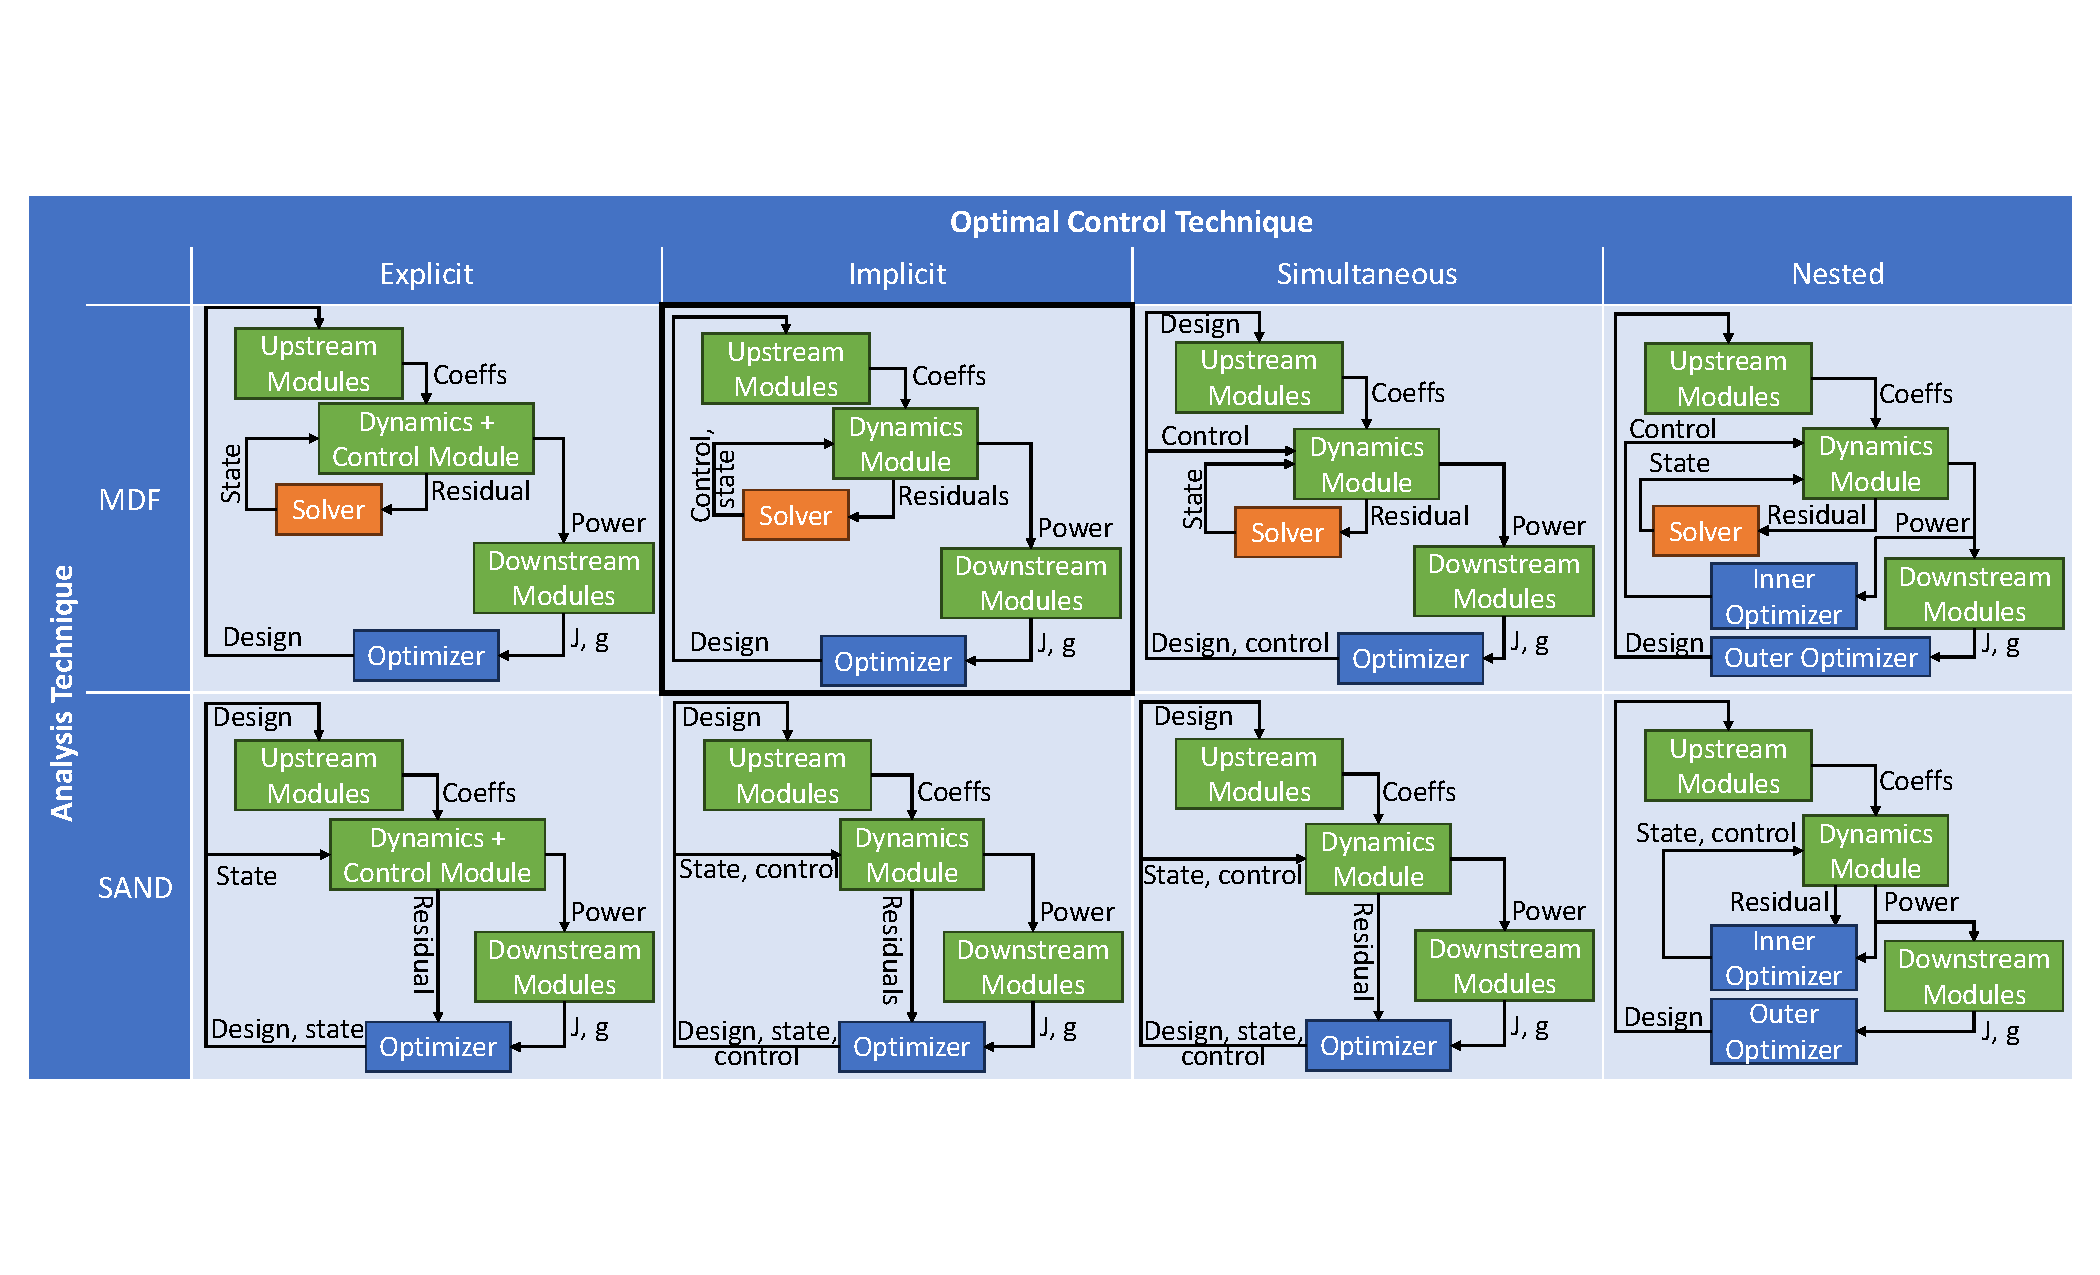
\includegraphics[width=1.1\linewidth]{../renewable-energy-mdo/figs/control_analysis_flowcharts_2.pdf}
\caption{Optimization architectures organized by analysis method (MDF and SAND) and control method (explicit, implicit, simultaneous, and nested).}
\label{fig:control-arch}
\end{figure}